Last class we introduced the concept of counting paths. We learned three methods (I will do the last method next class) to count paths:
\begin{itemize}
    \item Brute force 
    \item Numbering the vertices
    \item Using word arrangements (e.g. how many ways can you arrange ``RRUUU'')
\end{itemize}
Obviously, brute force methods are not very efficient and have a high probability of having an error.

As for numbering the vertices, the way they work is that you can always consider a snapshot of the grid. Let's take the following example.

\begin{problem}
How many ways are there to walk from $A$ to $B$ if I can only move up or right?
\begin{center}
\begin{tikzpicture}
		\draw (0,0) grid (2,2);
		\node (a) at (-0.2, 0) {$A$}; 
		\node (b) at (2.2, 2) {$B$}; 
\end{tikzpicture}
\end{center}
\end{problem}

We first consider this smaller problem: how many ways can I get from $A$ to $A_3$?
\begin{center}
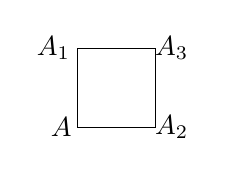
\begin{tikzpicture}
		\draw (0,0) grid (1,1);
		\node (a) at (-0.2, 0) {$A$}; 
		\node (a1) at (-0.3, 1) {$A_1$};
		\node (a2) at (1.2, 0) {$A_2$};
		\node (a3) at (1.2, 1) {$A_3$};
	\end{tikzpicture}
\end{center}
We clearly see that to get from $A \rightarrow A_1$, there is only one way (up), and from $A \rightarrow A_2$, there is only one way (right). So we mark ``1'' onto those vertices, indicating that ``there is 1 way to move from $A$ to those vertices''.
\begin{center}
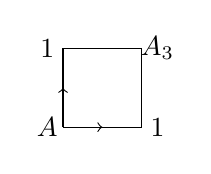
\begin{tikzpicture}
		\draw (0,0) grid (1,1);
		\draw[->] (0,0) -- (0, 0.5);
		\draw[->] (0,0) -- (0.5, 0);
		\node (a) at (-0.2, 0) {$A$}; 
		\node (a1) at (-0.2, 1) {$1$};
		\node (a2) at (1.2, 0) {$1$};
		\node (a3) at (1.2, 1) {$A_3$};
	\end{tikzpicture}
\end{center}
We now focus on the point $A_3$. I know in this example it's obvious that there are two ways to get from $A$ to $A_3$, but here we are going to view it in another way. Since there was one way to get to $A_1$ and one way to get to $A_2$, there must be $A_1+A_2$ ways to get to $A_3$, because those two vertices are the only two points where a person can pass through to get to $A_3$.
\begin{center}
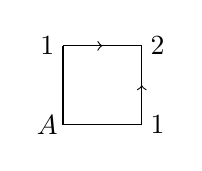
\begin{tikzpicture}
		\draw (0,0) grid (1,1);
		\draw[->] (0,1) -- (0.5, 1);
		\draw[->] (1,0) -- (1, 0.5);
		\node (a) at (-0.2, 0) {$A$}; 
		\node (a1) at (-0.2, 1) {$1$};
		\node (a2) at (1.2, 0) {$1$};
		\node (a3) at (1.2, 1) {$2$};
	\end{tikzpicture}
\end{center}

And here is the generalization, given any grid of $1\times 1$ where the only legal moves are up and right (these rules can be generalized too), the total number of paths into the upper right hand corner vertex is the sum of the number of ways to reach the two vertices that precede it. The figure that illustrates this fact is shown below.
\begin{center}
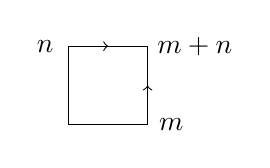
\begin{tikzpicture}
		\draw (0,0) grid (1,1);
		\draw[->] (0,1) -- (0.5, 1);
		\draw[->] (1,0) -- (1, 0.5);
		\node (a1) at (-0.3, 1) {$n$};
		\node (a2) at (1.3, 0) {$m$};
		\node (a3) at (1.6, 1) {$m+n$};
	\end{tikzpicture}
\end{center}
Using this fact, we can fill in our grid from the original problem.
\begin{center}
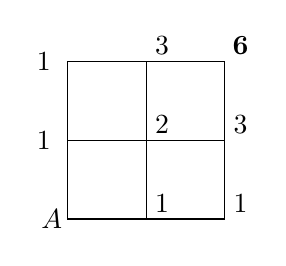
\begin{tikzpicture}
		\draw (0,0) grid (2,2);
		\node (a) at (-0.2, 0) {$A$}; 
		\node (a1) at (-0.3, 1) {$1$};
		\node (a1) at (-0.3, 2) {$1$};
		\node (a2) at (1.2, 0.2) {$1$};
		\node (a3) at (1.2, 1.2) {$2$};
		\node (a3) at (1.2, 2.2) {$3$};
		\node (a2) at (2.2, 0.2) {$1$};
		\node (a3) at (2.2, 1.2) {$3$};
		\node (a3) at (2.2, 2.2) {\textbf{6}};
	\end{tikzpicture}
\end{center}

And we see our answer is 6 total paths. Make sure you understand how to do these grids using this method because this works for \textit{any} path. The more efficient counting method with arranging moves only works for certain grids and will be covered next class.

\subsection{Problems}

\begin{problem}
How many ways are there to walk from $A$ to $B$ if I can only move up or right?
\begin{center}
\begin{tikzpicture}
		\draw (0,0) grid (4,3);
		\node (a) at (-0.3, 0) {$A$}; 
		\node (b) at (4.2, 3) {$B$}; 
\end{tikzpicture}
\end{center}
\end{problem}

\begin{problem}
If a ladybug walks on the segments of the diagram from point A to point B moving only to the right or downward, how many distinct paths are possible?  (\textit{MATHCOUNTS})
\begin{center}
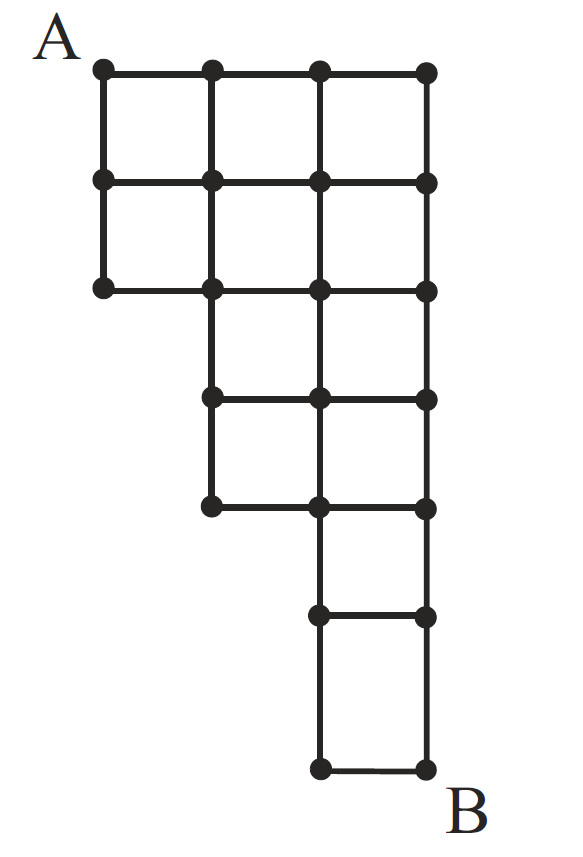
\includegraphics[width=2in]{path}
\end{center}
\end{problem}

\begin{problem}
In the figure below, how many ways are there to select 5 bricks, one in each row, such that any two bricks in adjacent rows are adjacent? (\textit{HMMT})
\begin{center}
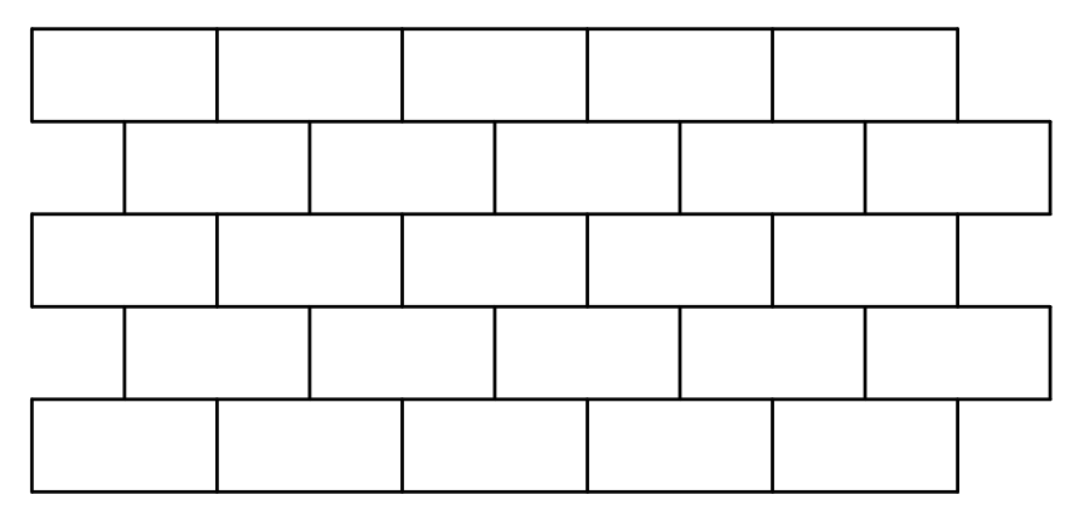
\includegraphics[width=3in]{grid}
\end{center}
\end{problem}

\begin{problem}
How many ways are there to walk from $A$ to $C$ if I must go through point $B$? (hint...you can try labeling the vertices like normal or split the problem into two parts)
\begin{center}
\begin{tikzpicture}
		\draw (0,0) grid (5,3);
		\node (a) at (-0.3, 0) {$A$}; 
		\node (b) at (3.2, 2.2) {$B$};
		\node (b) at (5.2, 3.0) {$C$};
\end{tikzpicture}
\end{center}
\end{problem}

\subsection{A Teaser}
I will leave you guys with an opportunity to see how we can find an easier way to count the number of paths on a grid. Consider any grid of $m\times n$. Then in order to make it from one corner to the other, we must move right exactly $m$ times and up exactly $n$ times. If you want to see this in action, try drawing paths in the diagram below and writing out the letters to the paths you make. For example, in the diagram below, 

\begin{center}
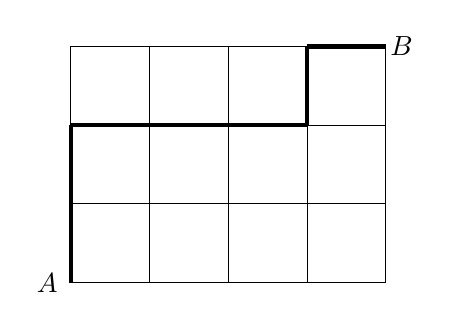
\begin{tikzpicture}
		\draw (0,0) grid (4,3);
		\node (a) at (-0.3, 0) {$A$}; 
		\node (b) at (4.2, 3) {$B$}; 
		\draw[ultra thick] (0,0) -- (0,2);
		\draw[ultra thick] (0,2) -- (3,2);
		\draw[ultra thick] (3,2) -- (3,3);
		\draw[ultra thick] (3,3) -- (4,3);
\end{tikzpicture}
\end{center}

the path can be denoted by the sequence ``UURRRUR''. Using this information, see if you can derive the formula for the number of paths from corner to corner in a $m\times n$ grid.